% Credits are indicated where needed. The general idea is based on a template by Vel (vel@LaTeXTemplates.com) and Frits Wenneker.

\documentclass[11pt, a4paper]{article} % General settings in the beginning (defines the document class of your paper)
% 11pt = is the font size
% A4 is the paper size
% “article” is your document class

%----------------------------------------------------------------------------------------
%	Packages
%----------------------------------------------------------------------------------------

% Necessary
\usepackage[german,english]{babel} % English and German language 
\usepackage{hyperref} % URL
\usepackage{subfig} %two figure
\usepackage{listings} % Insert code
\usepackage{float} % figure at the correct position
\usepackage{lipsum}
\usepackage{mwe}
\usepackage{booktabs} % Horizontal rules in tables 
% For generating tables, use “LaTeX” online generator (https://www.tablesgenerator.com)
\usepackage{comment} % Necessary to comment several paragraphs at once
\usepackage[utf8]{inputenc} % Required for international characters
\usepackage[T1]{fontenc} % Required for output font encoding for international characters

% Might be helpful
\usepackage{amsmath,amsfonts,amsthm} % Math packages which might be useful for equations
\usepackage{tikz} % For tikz figures (to draw arrow diagrams, see a guide how to use them)
\usepackage{tikz-cd}
\usetikzlibrary{positioning,arrows} % Adding libraries for arrows
\usetikzlibrary{decorations.pathreplacing} % Adding libraries for decorations and paths
\usepackage{tikzsymbols} % For amazing symbols ;) https://mirror.hmc.edu/ctan/graphics/pgf/contrib/tikzsymbols/tikzsymbols.pdf 
\usepackage{blindtext} % To add some blind text in your paper


%---------------------------------------------------------------------------------
% Additional settings
%---------------------------------------------------------------------------------

%---------------------------------------------------------------------------------
% Define your margins
\usepackage{geometry} % Necessary package for defining margins

\geometry{
	top=2cm, % Defines top margin
	bottom=2cm, % Defines bottom margin
	left=2.2cm, % Defines left margin
	right=2.2cm, % Defines right margin
	includehead, % Includes space for a header
	%includefoot, % Includes space for a footer
	%showframe, % Uncomment if you want to show how it looks on the page 
}

\setlength{\parindent}{15pt} % Adjust to set you indent globally 

%---------------------------------------------------------------------------------
% Define your spacing
\usepackage{setspace} % Required for spacing
% Two options:
\linespread{1.5}
%\onehalfspacing % one-half-spacing linespread

%----------------------------------------------------------------------------------------
% Define your fonts
\usepackage[T1]{fontenc} % Output font encoding for international characters
\usepackage[utf8]{inputenc} % Required for inputting international characters

\usepackage{XCharter} % Use the XCharter font


%---------------------------------------------------------------------------------
% Define your headers and footers

\usepackage{fancyhdr} % Package is needed to define header and footer
\pagestyle{fancy} % Allows you to customize the headers and footers

%\renewcommand{\sectionmark}[1]{\markboth{#1}{}} % Removes the section number from the header when \leftmark is used

% Headers
\lhead{} % Define left header
\chead{\textit{}} % Define center header - e.g. add your paper title
\rhead{} % Define right header

% Footers
\lfoot{} % Define left footer
\cfoot{\footnotesize \thepage} % Define center footer
\rfoot{ } % Define right footer

%---------------------------------------------------------------------------------
%	Add information on bibliography
\usepackage{natbib} % Use natbib for citing
\usepackage{har2nat} % Allows to use harvard package with natbib https://mirror.reismil.ch/CTAN/macros/latex/contrib/har2nat/har2nat.pdf

% For citing with natbib, you may want to use this reference sheet: 
% http://merkel.texture.rocks/Latex/natbib.php

%---------------------------------------------------------------------------------
% Add field for signature (Reference: https://tex.stackexchange.com/questions/35942/how-to-create-a-signature-date-page)
\newcommand{\signature}[2][5cm]{%
  \begin{tabular}{@{}p{#1}@{}}
    #2 \\[2\normalbaselineskip] \hrule \\[0pt]
    {\small \textit{Signature}} \\[2\normalbaselineskip] \hrule \\[0pt]
    {\small \textit{Place, Date}}
  \end{tabular}
}
%---------------------------------------------------------------------------------
%	General information
%---------------------------------------------------------------------------------
\title{Deep Learning Final Project Report} % Adds your title
%\author
%{
%    \name{Alfons Hwu} % Add your first and last name
%    %\thanks{} % Adds a footnote to your title
%    \\
%    \institution{0416324, Dept of Computer Science NCTU} % Adds your institution
%}



%---------------------------------------------------------------------------------
%	Define what’s in your document
%---------------------------------------------------------------------------------
\begin{document}


% If you want a cover page, uncomment "%---------------------------------------------------------------------------------
% Cover page
%---------------------------------------------------------------------------------

% Here are more templates for other cover pages: https://www.latextemplates.com/cat/title-pages

% This example is based on this cover page example: https://www.latextemplates.com/template/academic-title-page

\begin{titlepage} % Starts new environment where the page number is not displayed and the count starts at 1 for the next page

%------------------------------------------------
%	Institutional information
%------------------------------------------------
	
\begin{minipage}{0.4\textwidth} % Begins new environment (like a text box)
    \begin{flushleft} % Sets environment on the left side of the paper
    \large
    National Chiao Tung University\\ % Add your institution
    Spring 2019 \\ % Add term
    Deep Learning \\ % Add course title
    Instructor: Jen-Tsung Chien\\ % Add instructor/supervisor name 
    \end{flushleft}
\end{minipage}
	
\vspace*{2in} % Adds some space in-between
	
\center % Centre everything on the page

%------------------------------------------------
%	Main part
%------------------------------------------------
	
{\huge\bfseries Deep Learning HW2 Report}\\[0.4cm] % Add your paper title {\large\today}\\[0.4cm] % Add date (current day)
Alfons Hwu \\ % Add your name
Student ID: 0416324\\
\vfill % Adds additional space

%------------------------------------------------
%	General information about the author
%------------------------------------------------

\vfill % Adds additional space

alfons.cs04@g2.nctu.edu.tw \\ % Add your contact info
Dept of Computer Science \\ % Add info about your program
Writing with \LaTeX  on Overleaf

\vfill % Adds additional space

%------------------------------------------------
%	Word count
%------------------------------------------------

\vfill % Adds additional space
	
\end{titlepage}" and uncomment "\begin{comment}" and "\end{comment}" to comment the following lines
%---------------------------------------------------------------------------------
% Cover page
%---------------------------------------------------------------------------------

% Here are more templates for other cover pages: https://www.latextemplates.com/cat/title-pages

% This example is based on this cover page example: https://www.latextemplates.com/template/academic-title-page

\begin{titlepage} % Starts new environment where the page number is not displayed and the count starts at 1 for the next page

%------------------------------------------------
%	Institutional information
%------------------------------------------------
	
\begin{minipage}{0.4\textwidth} % Begins new environment (like a text box)
    \begin{flushleft} % Sets environment on the left side of the paper
    \large
    National Chiao Tung University\\ % Add your institution
    Spring 2019 \\ % Add term
    Deep Learning \\ % Add course title
    Instructor: Jen-Tsung Chien\\ % Add instructor/supervisor name 
    \end{flushleft}
\end{minipage}
	
\vspace*{2in} % Adds some space in-between
	
\center % Centre everything on the page

%------------------------------------------------
%	Main part
%------------------------------------------------
	
{\huge\bfseries Deep Learning HW2 Report}\\[0.4cm] % Add your paper title {\large\today}\\[0.4cm] % Add date (current day)
Alfons Hwu \\ % Add your name
Student ID: 0416324\\
\vfill % Adds additional space

%------------------------------------------------
%	General information about the author
%------------------------------------------------

\vfill % Adds additional space

alfons.cs04@g2.nctu.edu.tw \\ % Add your contact info
Dept of Computer Science \\ % Add info about your program
Writing with \LaTeX  on Overleaf

\vfill % Adds additional space

%------------------------------------------------
%	Word count
%------------------------------------------------

\vfill % Adds additional space
	
\end{titlepage}

\date{June 20, 2019}
\begin{comment}
\end{comment}
\maketitle{} %Print your title, author name and date; comment if you want a cover page 

%----------------------------------------------------------------------------------------
% Introduction
%----------------------------------------------------------------------------------------
\setcounter{page}{1} % Sets counter of page to 1

\section{Introduction} % Add a section title
\\ Here we introduce an
artificial system based on a Convolutional Neural Network that creates artistic images
of high perceptual quality. The system uses neural representations to separate and recombine content and style of arbitrary images, providing a neural
algorithm for the creation of artistic images. 
\\ In this project, we hope to "translate" the image from "young face" to "old face" and vice versa by using the "Neuron Style Transfer" mentioned in \url{https://arxiv.org/abs/1508.06576} with vgg network and some self-designed model.
\section{Model Architecture}
\\ The architecture is simple, we have three images, S represents the style image, C represents the content image and G represent the synthesized image to be generated.
\begin{figure}[H]
    \centering
    \subfloat[Model architecture]{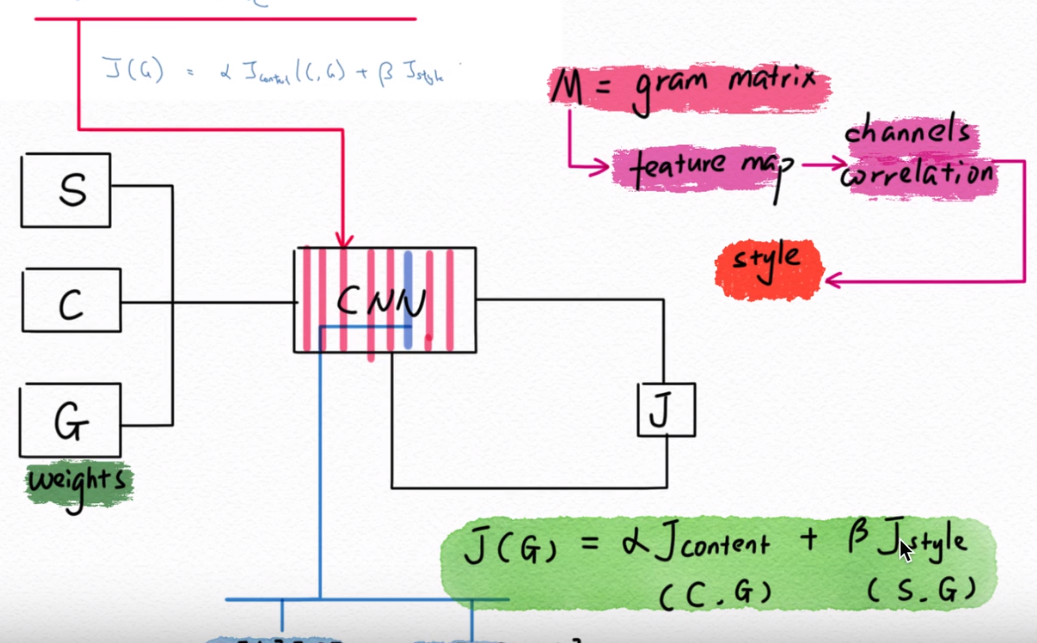
\includegraphics[scale = 0.3]{Final_Project/arch.png}\label{fig:f1}}
    \caption{Model}
\end{figure}
\\ The CNN model used is the pretrained VGG-19 network, which is a convolutional neural network that is trained on more than a million images from the ImageNet database. The network is 19 layers deep and trained on millions of images. Because of which it is able to detect high-level features in an image. 
\\ During the convolution procedure, features in images can be filtered out and they are called "feature maps". We may calculate the content loss and style loss respectively with $p$ being the content image, $a$ being the art style image, $x$ being the generated, synthesized image. 
\\ Hence, overall loss to be {\Large $$L_{total}(p, a, x) = \alpha L_{content}(p, x) + \beta L_{style}(a, x)$$}
\section{Understand the math behind the loss}
\\ Reference and revised from \url{https://arxiv.org/abs/1508.06576} page 10 to 12
\subsection{The loss of content}
\\ A layer with $N_{l}$ distinct filters has $N_{l}$ feature maps each of size $M_{l}$
, where $M_{l}$ is the height times the width of the feature map (magnitude).
\\ So the responses in a layer $l$ can be stored in a matrix $F_{l} \in R^{N_l \times M_l}$ where $F^{l}_{ij}$ is the activation of the $i^{th}$ filter at position $j$ in layer $l$ and the same is true for $P^l_{ij}$ 
\\ Let $p$ and $x$ be be the original image and the image that is generated. $P^{l}$, $F^{l}$ being their respective feature representation in layer $l$ after extracted by convolutional filter.
\\ We may thus use the mean square error to compare the original content image and generated image \textbf{pixel-wisely.}
\\ {\Large $$L_{content}(p, x, l) = \frac{1}{2} \sum_{i, j}(F^{l}_{ij} - P^l_{ij})^2$$}

\subsection{The loss of style}
\\ On top of the CNN responses in each layer of the network we built a style representation
that computes the correlations between the different filter responses, where the expectation is
taken over the spatial extend of the input image. These feature correlations are given by the
Gram matrix $G_{l} \in R^{N_l \times N_l}$
, where $G{l}_{ij}$ is the inner product between the vectorised feature map $i$ and $j$ in layer $l$:
\\ {\Large $$G^{l}_{ij} = \sum_{k}(F^{l}_{ik} - F^l_{jk})$$}
\\ Finally we use gradient descent to minimize the difference between original style image $a$ and generated image $x$ and $A^l$ and $G^l$ being their respective style representations in layer $l$
\\ Total loss of style will be
\\ {\Large $$E_{l} = \frac{1}{4N^{2}_{l}M^2_{l}} \sum_{i, j}(G^{l}_{ij} - A^l_{ij})^2$$}
\\ {\Large Why does it work?, especially in the style loss.}
\\ First, try to optimize the content difference is quite in intuitive.
\\ Yet concerning the style loss,in order to capture the style of an image we would calculate how “correlated” these filters are to each other meaning how similar are these feature maps.
\\ Here the \textbf{Gram matrix} helps solve this problem, since it is defined as a set of vectors in an inner product space, which is the \textbf{Hermitian matrix} of inner products, whose entries are given by $G_{ij} = \langle V_{i}, V_{j}\rangle$
\\ If the dot-product across the activation of two filters is large then two channels are said to be correlated and if it is small then the images are un-correlated.
\\ 
\begin{figure}[H]
    \centering
    \subfloat[Reply]{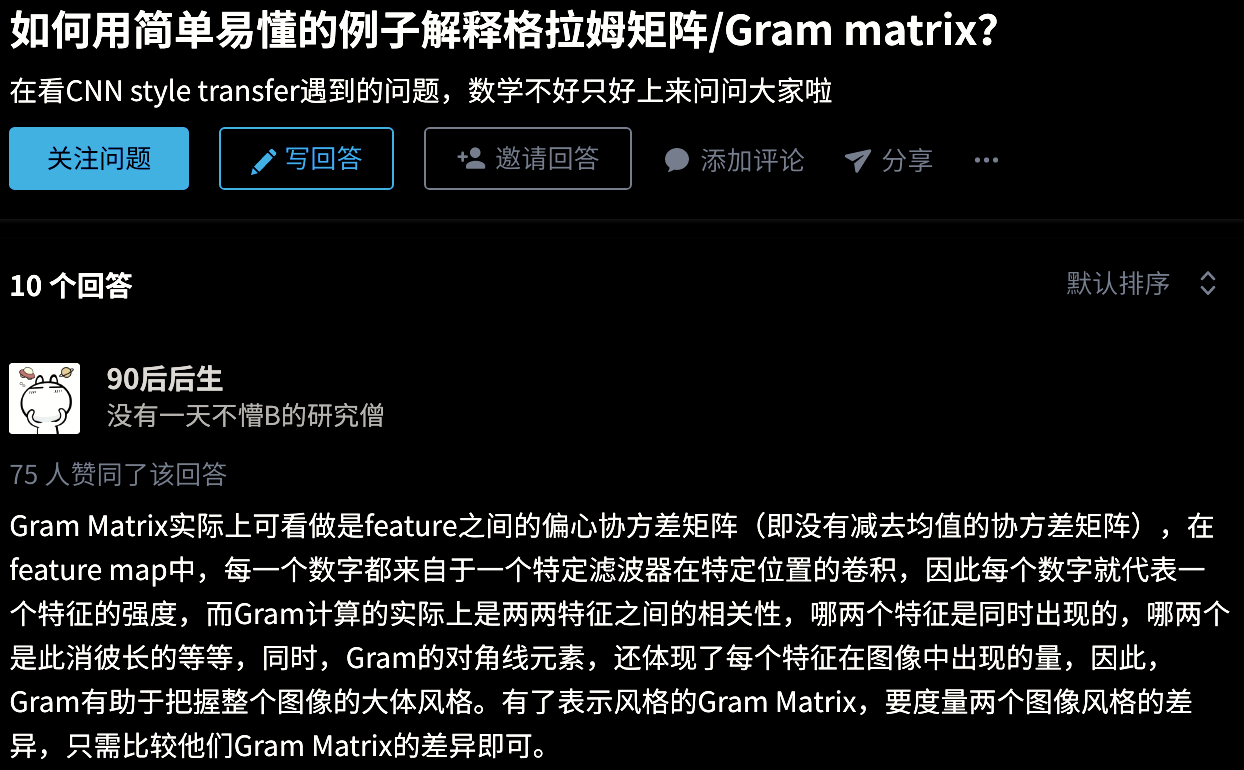
\includegraphics[scale = 0.3]{Final_Project/zhihu.png}\label{fig:f1}}
    \caption{Zhihu reply for understanding the gram matrix}
\end{figure}
\\ Based on the reply from \url{https://www.zhihu.com/question/49805962}
\\ $G^{l}_{ij} = \sum_{k}(F^{l}_{ik} - F^l_{jk})$ will go through each combination of inner-producted feature maps, either in the original image or generated image, consequently all the all vital features of images are represented.
\\ Cost function between style and generated image is the \textbf{square of difference between the Gram Matrix of the style Image with the Gram Matrix of generated Image.} $E_{l} = \frac{1}{4N^{2}_{l}M^2_{l}} \sum_{i, j}(G^{l}_{ij} - A^l_{ij})^2$
\\ Finally we will derive the total loss function $L_{total}(p, a, x) = \alpha L_{content}(p, x) + \beta L_{style}(a, x)$
\\ By adjusting the weight of $\alpha$ and $\beta$, we may either emphasize the style or content for the generated image.

\section{Dataset Description}
\\ We have collected some of the young face as the style image and old face as content image hoping to rejuvenile the old face. 
\section{Dataset Preprocessing}
\section{Result Evaluation}
\section{Group Work Distribution}
\\ 0416324: NN architecture, testing, shell scripting to automatically organize and train data / IO, writing this LaTeX report.
\\ 0416033: Organize data, checking output result and feedback to 0416324 and 0416045 to revise.
\\ 0416045: NN architecture, testing and ppt.
\\ 0416022: Make demo video, ppt
\section{Reference Data}
\item Neuron Style Algorithm: \url{https://arxiv.org/abs/1508.06576}
\item Neuron Style Superposition(famous paper by Li Fei-Fei from Stanford University) \url{https://arxiv.org/abs/1508.06576}
\item Zhihu reply \url{https://www.zhihu.com/question/49805962}
\item Medium article 1 \url{https://hackernoon.com/how-do-neural-style-transfers-work-7bedaee0559a}
\item Medium article 2 \url{https://towardsdatascience.com/style-transfer-styling-images-with-convolutional-neural-networks-7d215b58f461}
\item Bilibili video tutorial \url{https://www.bilibili.com/video/av22581633/?p=41}
\item Quora reply \url{https://www.quora.com/What-is-Gram-matrix-What-is-its-significance-in-linear-algebra}
\end{document}